\documentclass[a4paper, 11pt]{article}
\usepackage[T1]{fontenc}
\usepackage[margin=2.5cm, nohead]{geometry}
\usepackage{palatino, url, multicol}
\usepackage{amssymb, graphicx, fancyhdr, latexsym, url, verbatim}
\usepackage{algorithm, algorithmic}
\usepackage{hyperref}
\usepackage{clrscode3e}
\usepackage[all]{xy}
\usepackage[english]{babel}
\usepackage{matlabScripts}
\usepackage[font=small,format=plain,labelfont=bf,up,textfont=it,up]{caption}
\usepackage{xspace}
%\usepackage{subfigure} % has to be loaded after caption to prevent clash Commented, because subfig is the newer (and presumably
% better) version of subfigure...
\usepackage{subfig}



\newcommand{\projectName}{ACHTBITS\xspace}
\newcommand{\projectAbbreviation}{Awesome
CHaradriiformes Toegepast BIrd Tracking System\xspace}
\newcommand{\bits}{BITS\xspace}
% xspace only puts a space where we want one!
\newcommand{\matlab}{\textsc{matlab}\xspace}

\addtolength{\footskip}{-90mm}
\addtolength{\headheight}{-05mm}
\addtolength{\headsep}{05mm}



\pagestyle{fancy}
\lhead{\projectName}
\rhead{\small \textsc{\projectAbbreviation}}
%\cfoot{\footnotesize \textit{ \projectAbbreviation}\\[0.1cm] \small \thepage}
%\cfoot{}
%\rfoot{\thepage}


\setlength{\parindent}{0pt}
\setlength{\parskip}{10pt}

\begin{document}

\newcommand{\HRule}{\rule{\linewidth}{0.5mm}}

\begin{titlepage}
\begin{center}

\includegraphics[width=1\textwidth]{uva}\\[0.5cm]

\HRule \\[0.2cm]
{ \huge \LARGE \textbf{\projectName}\\[0.1cm]
\large \textsc{\projectAbbreviation}
 \vspace{0.2cm}}
\HRule \\[0.4cm]
\Large \today

\vfill

\begin{tabular}{cccc}
Jesse Eisses & Sosha Happel & Maarten Inja & Maarten de Waard \\ 
6352189 & 6273831 & 5872464 & 5894883 
\end{tabular} \\[0.3cm]

\large \{mrtndwrd, maarten.inja, jesse.eisses, soshappel\}@gmail.com 
\end{center}
\end{titlepage}

%%{
%\begin{center}
%% Upper part of the page
%
%\textmd{Leren en Beslissen verslag}
%\vfill
%% Title
%{ \huge \textbf{ACHTBITS} \\\large \textsc{Awesome Charadriiformes Toegepast
%BIrd Tracking System}
%}\\[0.4cm]
%%\begin{center}
%\vfill
%By\\
%\vfill
%%\large\textbf{{Maarten de Waard \\ 5894883},  {Maarten Inja \\ 5872464},  {Jesse Eisses \\
%%6352189}, {Sosha Happel \\ 6273831}}
%\begin{tabular}{cccc}
%Jesse Eisses & Sosha Happel & Maarten Inja & Maarten de Waard \\ 
%6352189 & 6273831 & 5872464 & 5894883 
%\end{tabular}
%\vfill
%\{mrtndwrd, maarten.inja, jesse.eisses, soshappel\}@gmail.com
%%6352189 \and Sosha Happel\\ 6273831}
%\end{center}
%
%\end{titlepage}
%%}

%\thispagestyle{empty}
\vspace*{00mm}
\tableofcontents
\newpage


%%%%%%%%%%%%%%%% variables

\newcommand{\minimumSessionLengthMinutes}{60\xspace}
\newcommand{\resolutionRange}{$0.2$ - $\infty$\xspace}
\newcommand{\sessionSeparatorLengthMinutes}{15\xspace}
%% The current value of the timeThreshold given to awesomizeClusters.
\newcommand{\timeThreshold}{1200\xspace}
\newcommand{\windowSize}{20 minutes\xspace}

% sja, ik tiep hier maar wat hoor
\begin{abstract}
Using the data from the project of UvA-BITS, it is hard to classify the behavior of the sea gull above the North Sea. 
There is GPS data available and sometimes even accelerometer data but it 
remains troublesome to annotate data point by point. i

In this report we 
describe how we cluster data using histograms. We also describe the annotation
tool we built, with which we can annotate clustered data points more easily. 
\end{abstract}

\section{Introduction}
UvA Bird Tracking System\footnote{\url{http://www.uva-bits.nl/} } is a research 
project that studies the behavior of
birds. 
In contrast to some other birds that are being tracked the Sea Gull flies above the 
sea where it is a lot harder to watch and see what it is doing. We have data available
collected by a small device (see figure \ref{fig:gpsDevice}) that can be attached to 
the back of a bird. 

\begin{figure}
    \center
    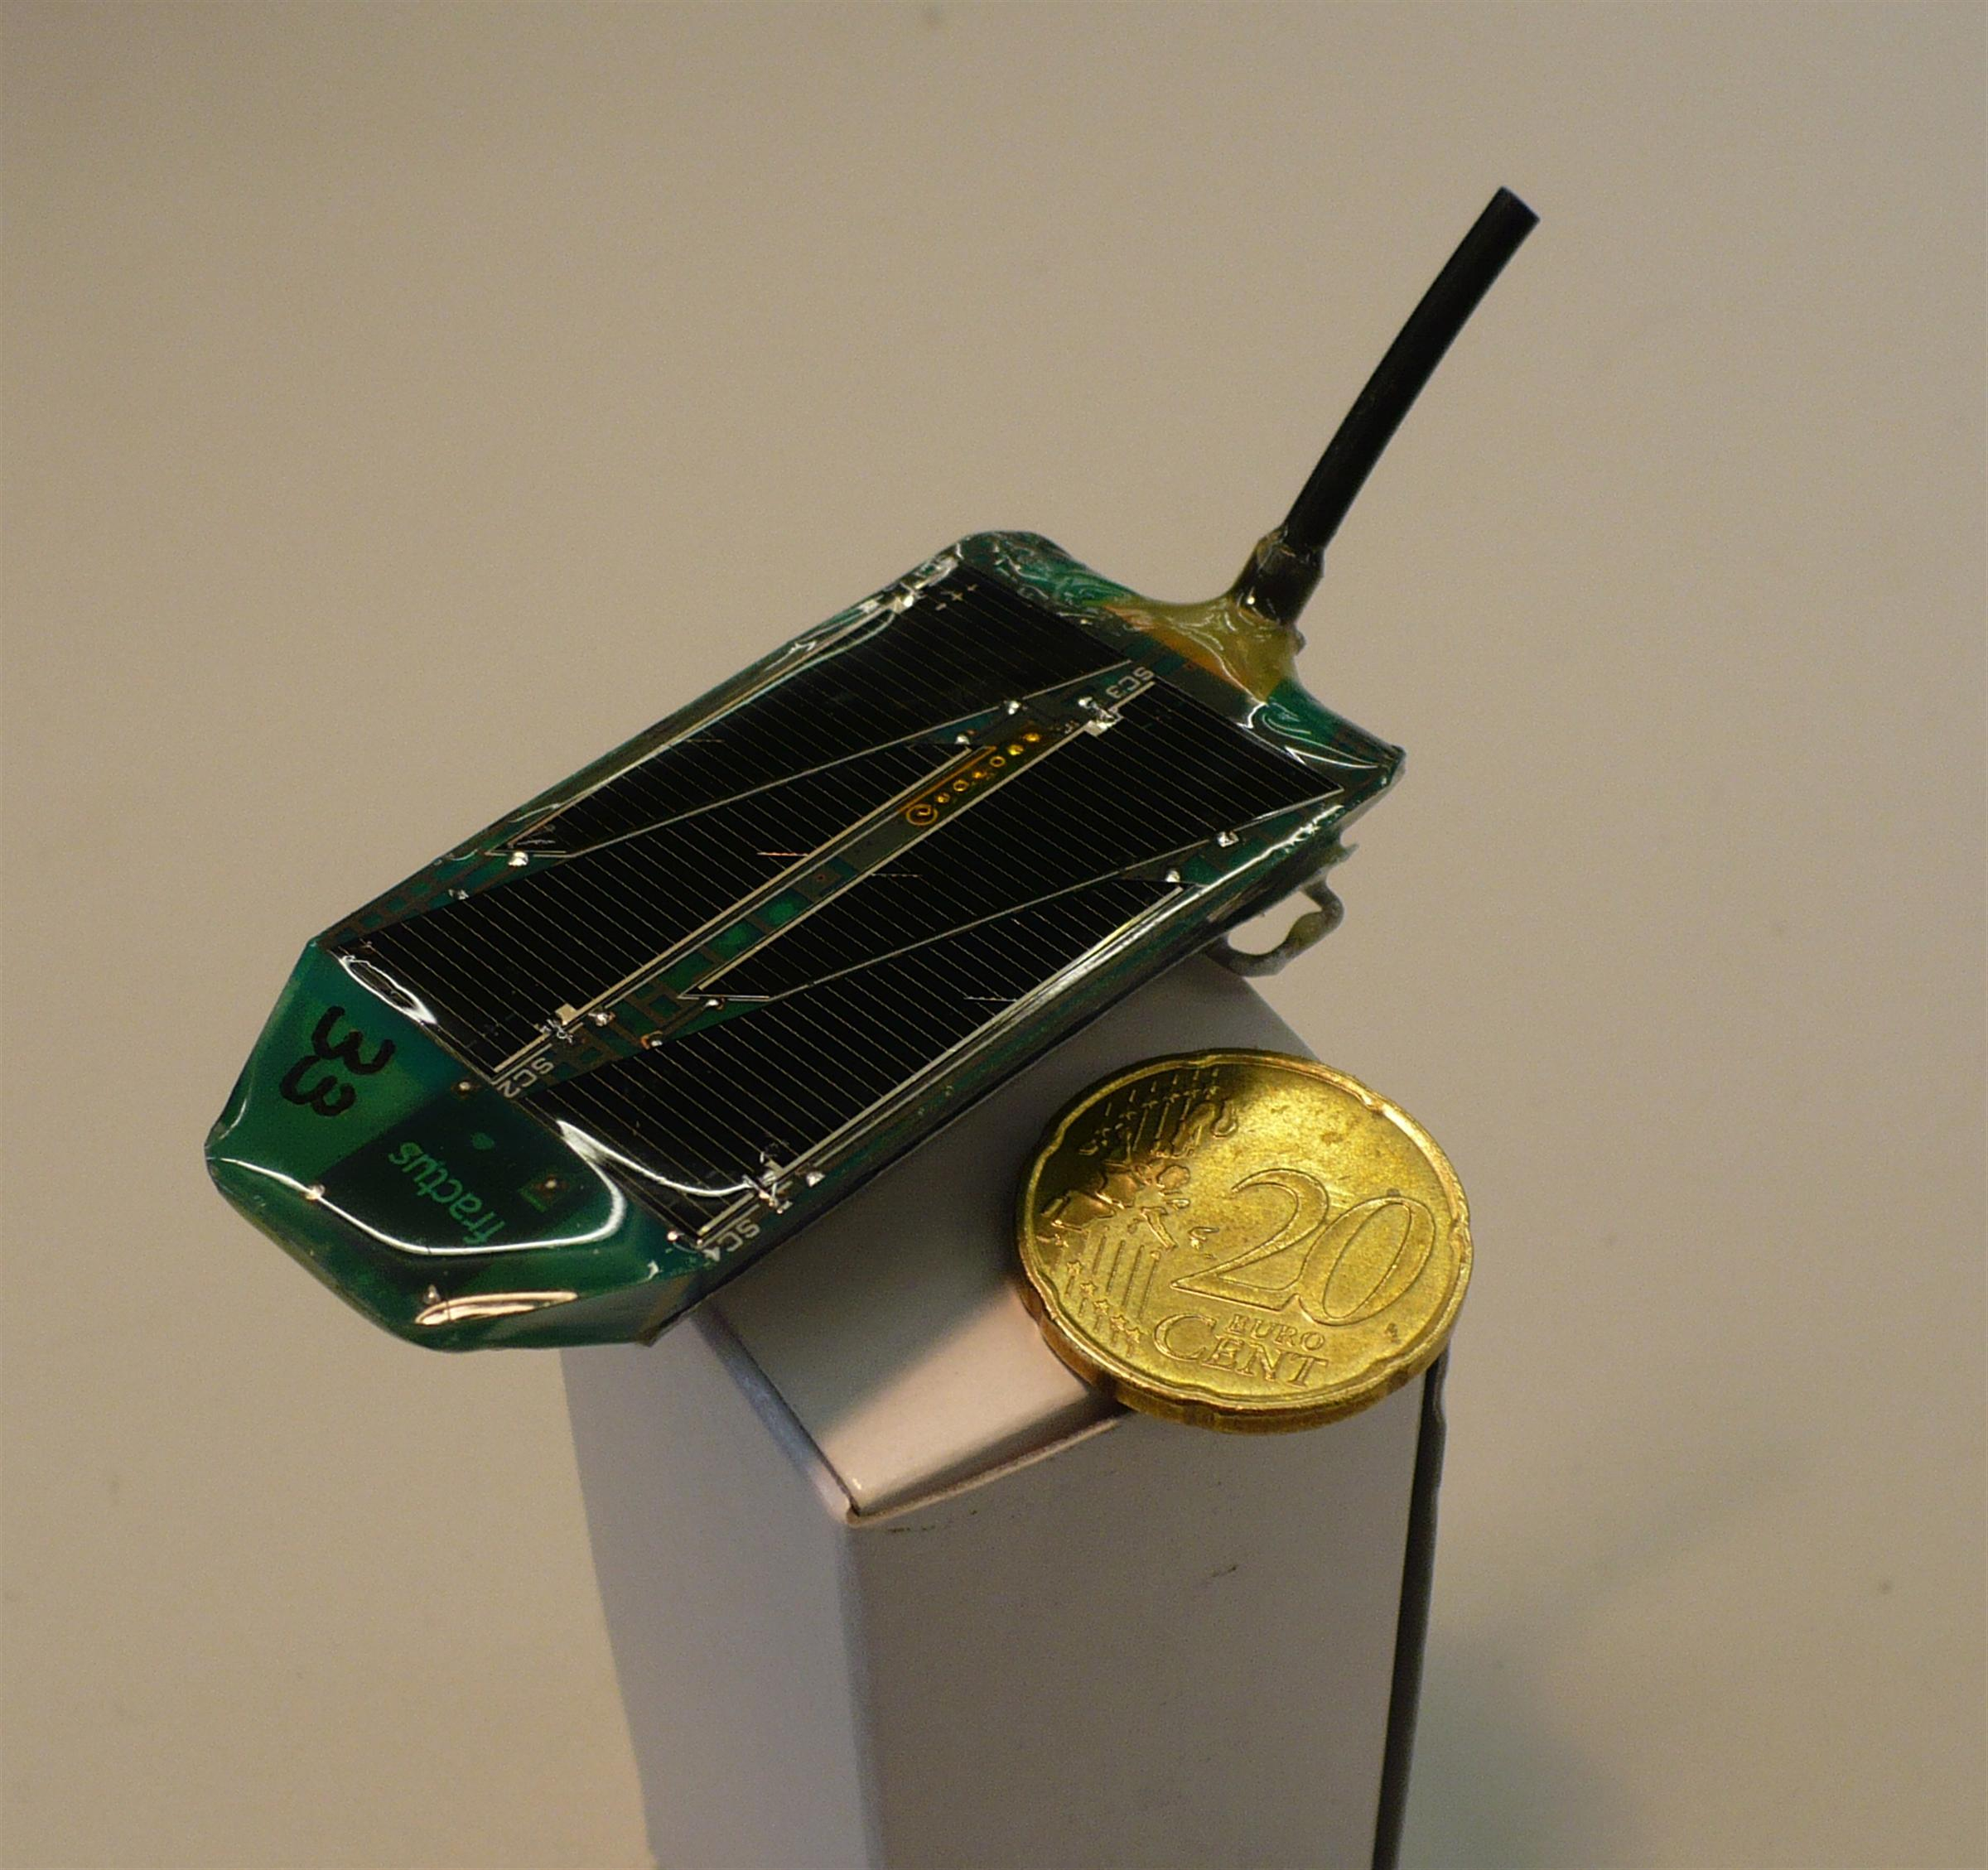
\includegraphics[width=7cm]{device}
    \caption{A small GPS device that can also transmit accelerometer data and some other
information}
    \label{fig:gpsDevice}
\end{figure}

The data, which consists of thousands of data points, is hard to read and to annotate. 
There are tools that can rewrite the data to a format that can be read by Google Earth. 
Viewing this data in Google Earth is a bit helpful to get a general idea of what such 
a gull might be doing but it does not allow for easy manipulation of the data. 

During four weeks we worked to preprocess, cluster, annotate
and lastly: classify the data. 

% perhaps more about the (other) research goals




\section{Preprocessing}


%\section{Preprocessing}
The data we need to use is available from a database at the uva-bits website
\footnote{\url{https://public.flysafe.sara.nl/phppgadmin/} }. This database is often very slow 
and sometimes overloaded. This is why we downloaded all the data we required in one run. 
Before we can start in \matlab we preprocess this data to load only correct data
in it.

\subsection{Before Matlab}
\label{subsec:beforeMatlab}
Preprocessing of the data from a database dump is done in Java. Such data 
is checked for the following: 
\begin{enumerate}
    \item Is the data above the north sea? We are only interested in the birds behaviour 
    above the North Sea data from above the Wadden Sea or above Holland is removed.
    \item Is the data complete? If we require longitude and latitude every entry 
    without a value for these variables are excluded for the data for \matlab. 
    \item Is the data usable? Our method requires data to consist of long flights,
    not isolated data points. We call a sequence of useful data points a \textit{session}. 
    See subsection \ref{subsec:creatingSessions} for more details on sessions and how
    they are created.
\end{enumerate}

Furthermore the date time was rewritten to a time stamp. We wanted the time stamps to be 
as small as possible so instead of using standard Unix time we use \textit{seconds passed
since 
January 1 2008}. This could be done because the earliest data in the database was from after
this date. 

\subsection{Creating Sessions}
\label{subsec:creatingSessions}
As discussed in subsection \ref{subsec:beforeMatlab} a part of the script involves 
dividing the data points up in to sessions. Isolated data points should be excluded. 
When there is a too big of a time span between two data points, a new sessions should be 
created. Furthermore a session should not be too short and it should not contain too few
data points (the resolution of data points per minutes should be within a range of 
acceptable values). 

This has to be done because our method involves the detection of clusters and this
can only be done with an actual flight of the bird. 

We use the following parameters to define which sequences of data points can be called sessions: 
\begin{itemize}
    \item Total minutes described. This is currently set to \minimumSessionLengthMinutes minutes. Less than \minimumSessionLengthMinutes minutes of flight is not interesting.
    \item Range of resolution. We can filter for a range of data points per minutes. There is
no way to extract the same amount of information from low resolution data as from high 
resolution data. This is why we filter out the low resolution data. The resolution 
we now use is \resolutionRange data points per minute.
    \item The maximum amount of minutes between two data points. Sometimes the device
can't update at the preferred moments. We end a session at such a point because we need
the information of what the bird is doing \emph{all the time} to be able to cluster 
acceptably. 
\end{itemize}

A lot of data is thrown away because of these filters. About \textbf{90\%} of the data 
from the database is data we can not use because it is not above the North Sea, incomplete
or not in context with other data points (can't be put in a session). The parameters are  
responsible for 
some of these percentages. We chose these parameters because our client told us it is better
to use less data which we know is good than use more data which can be questionable. In 
other words, it does not matter that much that we end up with less data to learn from and
to classify. 

\subsection{GPS and accelerometer data}
\label{subsec:gpsAndAccelerometerData}
There is also a difference between GPS data and accelerometer data, namely: there are a lot
more GPS data points then there are accelerometer data points
(It seems that \textbf{25\%} of the GPS data also has accelerometer data).
This is why we create 
sessions using only
the GPS data. We later match the accelerometer data to GPS sessions. 

The output of this
script is $N$ comma separated GPS session files (containing GPS data that together makes
a session) and $M$ (with $0 <= M <= N$) comma separated accelerometer data files. \matlab
can easily match GPS data with accelerometer data using these files. 

 \subsection{Normalizing Height}
 The best way to distinguish flying from floating is, of course, by the height of the bird. Unfortunately the height calculated by the GPS is very unreliable\footnote{this has to do with triangularisation and switching of satellites}. The absolute value of the height is unusable (often the bird is flying 100 meters below the surface), but changes in height can be used on short intervals. In the preprocessing we will remove outliers from this data (large shifts in height, often because of a satellite switch) so we can later try to create features from it.

\begin{figure}[htb!]
 \begin{center}
 \subfloat {
  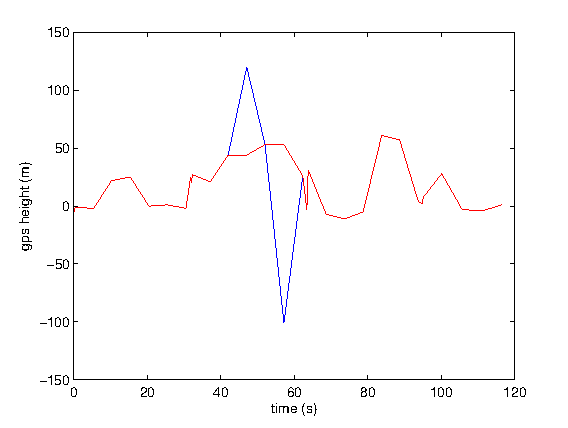
\includegraphics[scale=0.5]{heightnorm9}
 }
 \subfloat {
  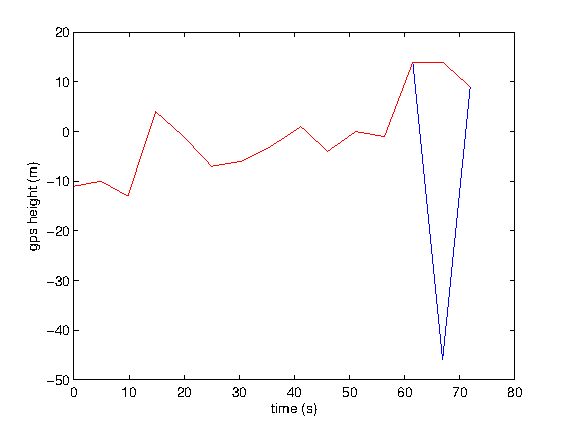
\includegraphics[scale=0.5]{heightnorm10}
 }
 \end{center}
 \caption{The blue line is the height from raw gps data, the red line is the normalized height.}
 \label{fig:heightnorm}
\end{figure}

We currently flatten height points in a cluster that are more than $3$ times the standard deviation away from the mean, which is a commonly used method\footnote{Sources:\\ http://en.wikipedia.org/wiki/Outlier\\ http://www.mathworks.nl/help/techdoc/data\_analysis/f0-7275.html} . Figure \ref{fig:heightnorm} shows some results. There is still a lot of noise left in the data, more experimenting will be needed to find a solution for this.





% Here we will discuss the preprocessing of the .csv files. This should consist
% of:
 % Describing how we only get the data above the north sea. Maybe an appendix
 % should be added on how the java script can (should) be run.
 
\section{Finding Clusters in the Data}
 % Describes how we find the peaks/clusters in the data (Maarten de Waard will
 % fill this in)
 This section will discuss how we find clusters in the raw data. 
 This is needed, to annotate these clusters, so we can later on use a
 learning algorithm on specified parts of the data.

% TODO: This piece of text is probably better suited elsewhere.
     Probably the most important of the GPS data we get from \bits are the X and Y
     position and speed of the bird. There are two speed entries in the database we
     use: One `instantaneous speed', the speed the bird has on the time of
     connecting to the GPS, calculated from two subsequent measurements, and a
     `trajectory speed', the speed the bird has between this, and the last
     measurement point. For clustering, we decided to use the latter, because this
     has a smaller error rate. Our assumption is that we can cluster the data good
     enough, by only looking at speed differences. Figure \ref{fig:speed} shows
     why.
 % TODO: Dit figuurtje maken. Ik kom er namelijk net achter dat de derivative
 % misschien niet exact doet wat we willen, omdat het speed1 en speed2 apart van
 % elkaar gebruikt. Een goeie hiervoor is device_535, sessie_000.

\begin{figure}
  \centering
  \subfloat[Speed of the bird.]{\label{fig:speed1}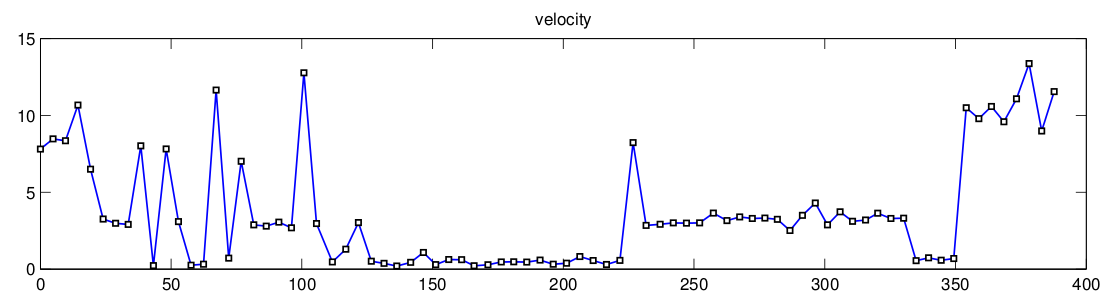
\includegraphics[width=0.8\textwidth]{speed1}} \\
  \subfloat[Difference in speed.]{\label{fig:speed2}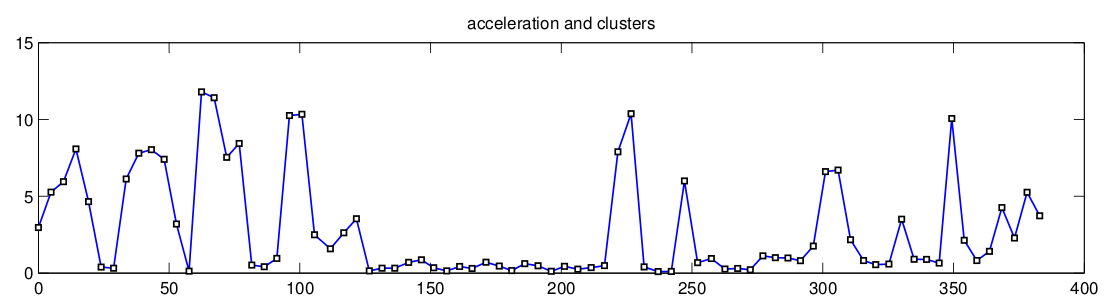
\includegraphics[width=0.8\textwidth]{speed2}} \\
  \caption{The difference is absolute because this makes finding peaks easier. The difference is sometimes a bit higher while the speed does not seem to differ at all. This means the bird changed directions.}
  \label{fig:speed}
\end{figure}

%\begin{figure}
%\centering
%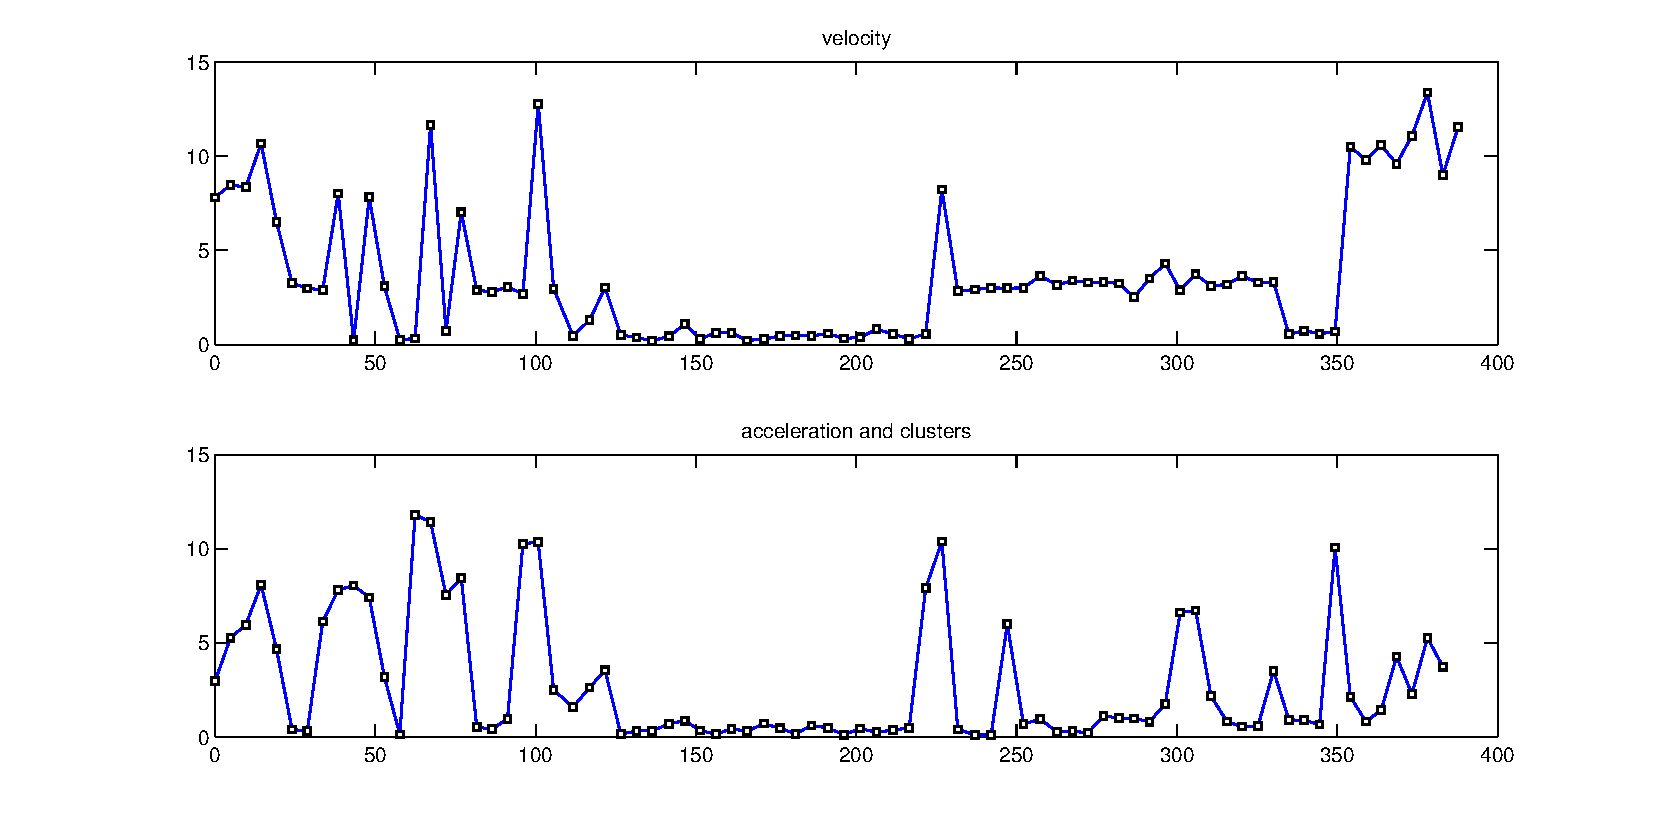
\includegraphics[width=.8\textwidth]{speed.pdf}
%\caption{The speed of the bird (above) and the difference in speed (under). As
%you can see, the difference is absolute (because this makes finding peaks
%easier). The difference is some times a bit higher, while the speed does not
%seem to differ at all. This means the bird changed his direction.}
%\label{fig:speed}
%\end{figure}

 As can be seen, the speed-difference is low on points where the bird is assumed
 to be flying or sitting on the water. In other points the speed differs a lot.
 On these places we can assume that the bird is foraging.

 We have tried two ways for finding clusters in the data. We started out with a
 quite straight-forward way, only looking at the speed differences of the bird.
 This worked quite well, but we needed some improvement. That is why we started
 working on a different version.

 This different version works on another basis: We create two histograms. One
 contains the trajectory speeds of the bird and the other contains the
 difference in the angle of the instantaneous speed. This means that we count
 how many times the speed or angle is between certain values, and represent that
 in an array with these counts. For further illustration see figure
 \ref{fig:histogram}.

\begin{figure}
\centering
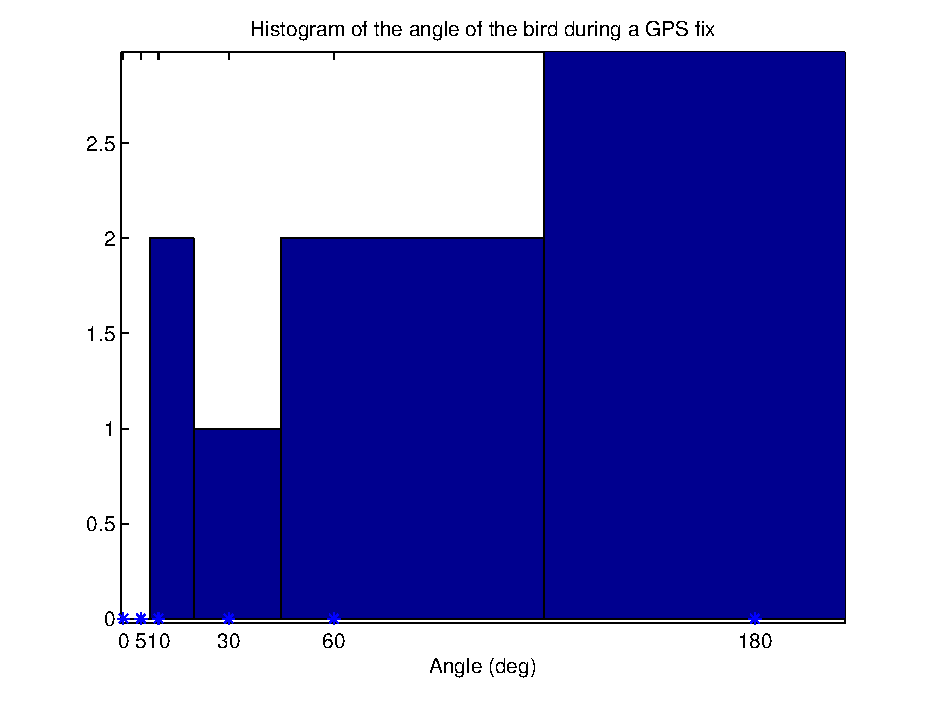
\includegraphics[width=.8\textwidth]{histogram.pdf}
\caption{Example of a histogram. The x-axis contains the bins. These are the
values in which the speeds could be. The height of the bars on the y-axis shows
us how many times in a certain time span the bird had a certain speed.}
\label{fig:histogram}
\end{figure}

\subsection{The First Way}
 \subsubsection{Finding Peaks}
 Clustering, in our case, starts with finding peaks in these speed differences.
 The peaks indicate a change in the bird's behavior, or indicate that the bird
 is foraging. Finding these peaks is done in two steps:

 \begin{itemize}
    \item Check where the value of the speed difference is bigger than a certain
    threshold.
    \item Loop through these differences and place a marker before the threshold
    is crossed upwards, or after it has been crossed downwards. 
 \end{itemize}
 
 This creates a representation of a peak by marking its left and right side.
 This comes in handy, because we do not want these speed differences in our
 clusters as they would add noise to the learning data.

 \subsubsection{Grouping Peaks}
 For grouping peaks, we created another algorithm. This algorithm looks at three
 characteristics.  
 \begin{enumerate}
 \item The time elapsed between two peaks
 \item The difference between the current time elapsed between peaks, and the
 current cluster's average
 \item The difference between the time elapsed between the first peak of the
 cluster, and the average of the rest of the cluster.
 \end{enumerate}
 This way we can find the `chaos clusters', because the time between the peaks
 in these clusters is always between a certain threshold (currently set on
 \timeThreshold seconds). 
 When a peak is too far from the  current average, this almost always indicates
 a change in behavior, so a new cluster should be started.this is done by the
 second and third characteristic specified above.

\subsection{The Second Method}
The second method we tried, relies on a bit more data. Apart from the trajectory
speed, now also the instantaneous speed is used. The trajectory speed is relevant for
the speed of the bird and now we use the instantaneous speed for finding the angle
at the time of the GPS fix. 

\begin{algorithm}
\begin{codebox}
\Procname{$\proc{histogramCompare}(Data, timeThreshold)$}
\li $exampleHists \gets getExampleHists()$
\li \For $i \gets 1 + timeThreshold$ \To $\attrib{Data}{length}$ 
\li \Do
    $currentHists \gets getHistograms(i-timeThreshold, i+timeThreshold)$
    \li $histogramValues(i) \gets \Sigma \left| currentHists - exampleHists \right|$
\End
\li \Return histogramValues
\end{codebox}
\caption{Comparing example histograms to our data}
\label{alg:hist}
\end{algorithm}

We take an example of each kind of behavior (floating, flying and foraging).
This example can be compared with a bit of the data we are
clustering. For this we loop over the data with a time window. This is probably
better explained in the pseudocode in algorithm \ref{alg:hist}.

When using this method, some problems have to be solved.

\subsubsection{Interpolating the Values}
The first problem we encounter is the difference in resolution of the data. This
would mean that when we are looking at high resolution data, and we compare it
with a low resolution example, line 4 of \ref{alg:hist} will not work. Therefore
we need to have exactly as many data points in the one, as in the other
histogram. 

This is easily achieved by interpolating the data. Since matlab has integrated
interpolation functions, we have chosen to interpolate with `Piecewise Cubic
Hermite Interpolating Polynomial (PCHIP)':, which is a bit more computationally
expensive than linear interpolation, but returns a smoother curve. This is
better, when using low resolution data, because it returns a bit smoother line.

\subsubsection{Comparing the Histograms}
As mentioned before, line 4 in algorithm \ref{alg:hist} compares two algorithms.
This returns a number close to zero, when the histograms are alike, and a high
number when they are different. Because this is not very intuitive, the program
recalculates this to percentages with equation \ref{eq:perc}.
\begin{equation}
\label{eq:perc}
percentage = 100 - \frac{Diff}{2 \sum Histogram} \times 100
\end{equation}

In this equation, Diff is the difference as calculated in algorithm
\ref{alg:hist} and the sum of a histogram is the count of all its entries. 

Now we have a percentage for each point, of how much it resembles each behavior.
A plot of this percentage is shown in the bottom of figure \ref{fig:clustering}.
This can be used to find clusters, because each time this differs, a new
cluster can be assumed to be starting.


\begin{figure}
  \centering
  \subfloat[Raw data of a session.]{\label{fig:clusteringRaw}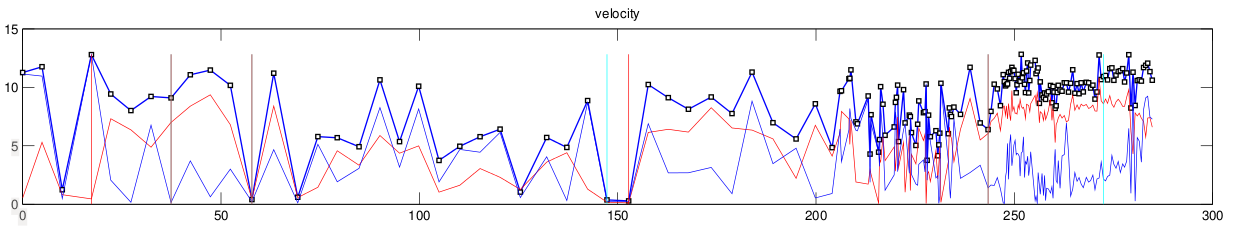
\includegraphics[width=0.8\textwidth]{clustersHists1}} \\
  \subfloat[Interpolated data of a session.]{\label{fig:clusteringInterpolated}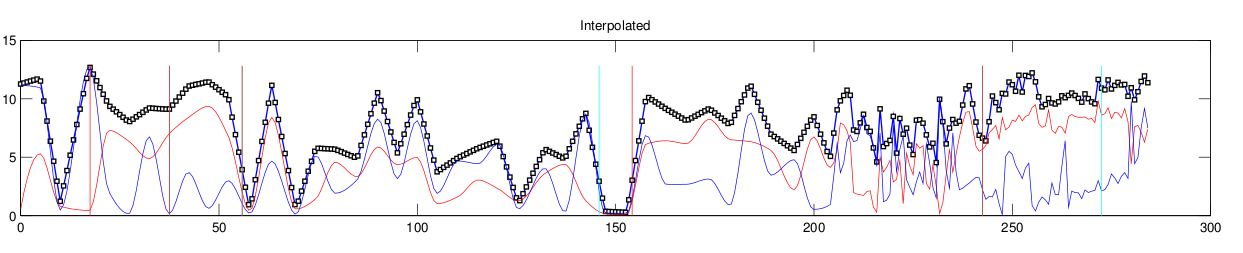
\includegraphics[width=0.8\textwidth]{clustersHists2}} \\
  \subfloat[Similarity of the flight to behavior percentages. Red indicates floating, green flying and blue hunting.]{\label{fig:clusteringHists}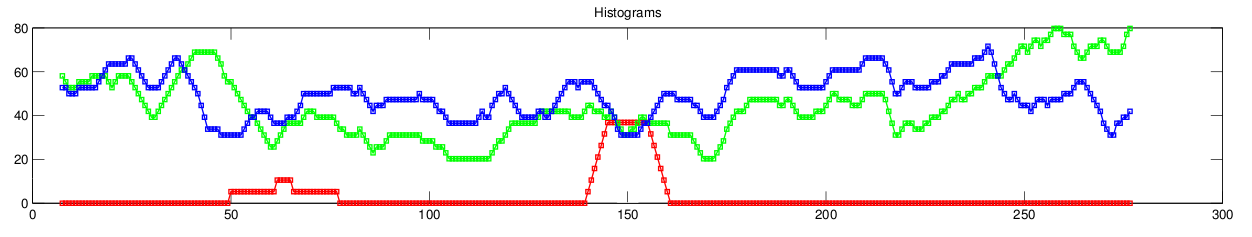
\includegraphics[width=0.8\textwidth]{clustersHists3}}
  \caption{Different plots of the clustering process. Red vertical bars indicate starts of clusters. Cyan vertical bars indicate ends of clusters.}
  \label{fig:clustering}
\end{figure}

%\begin{figure}
%\centering
%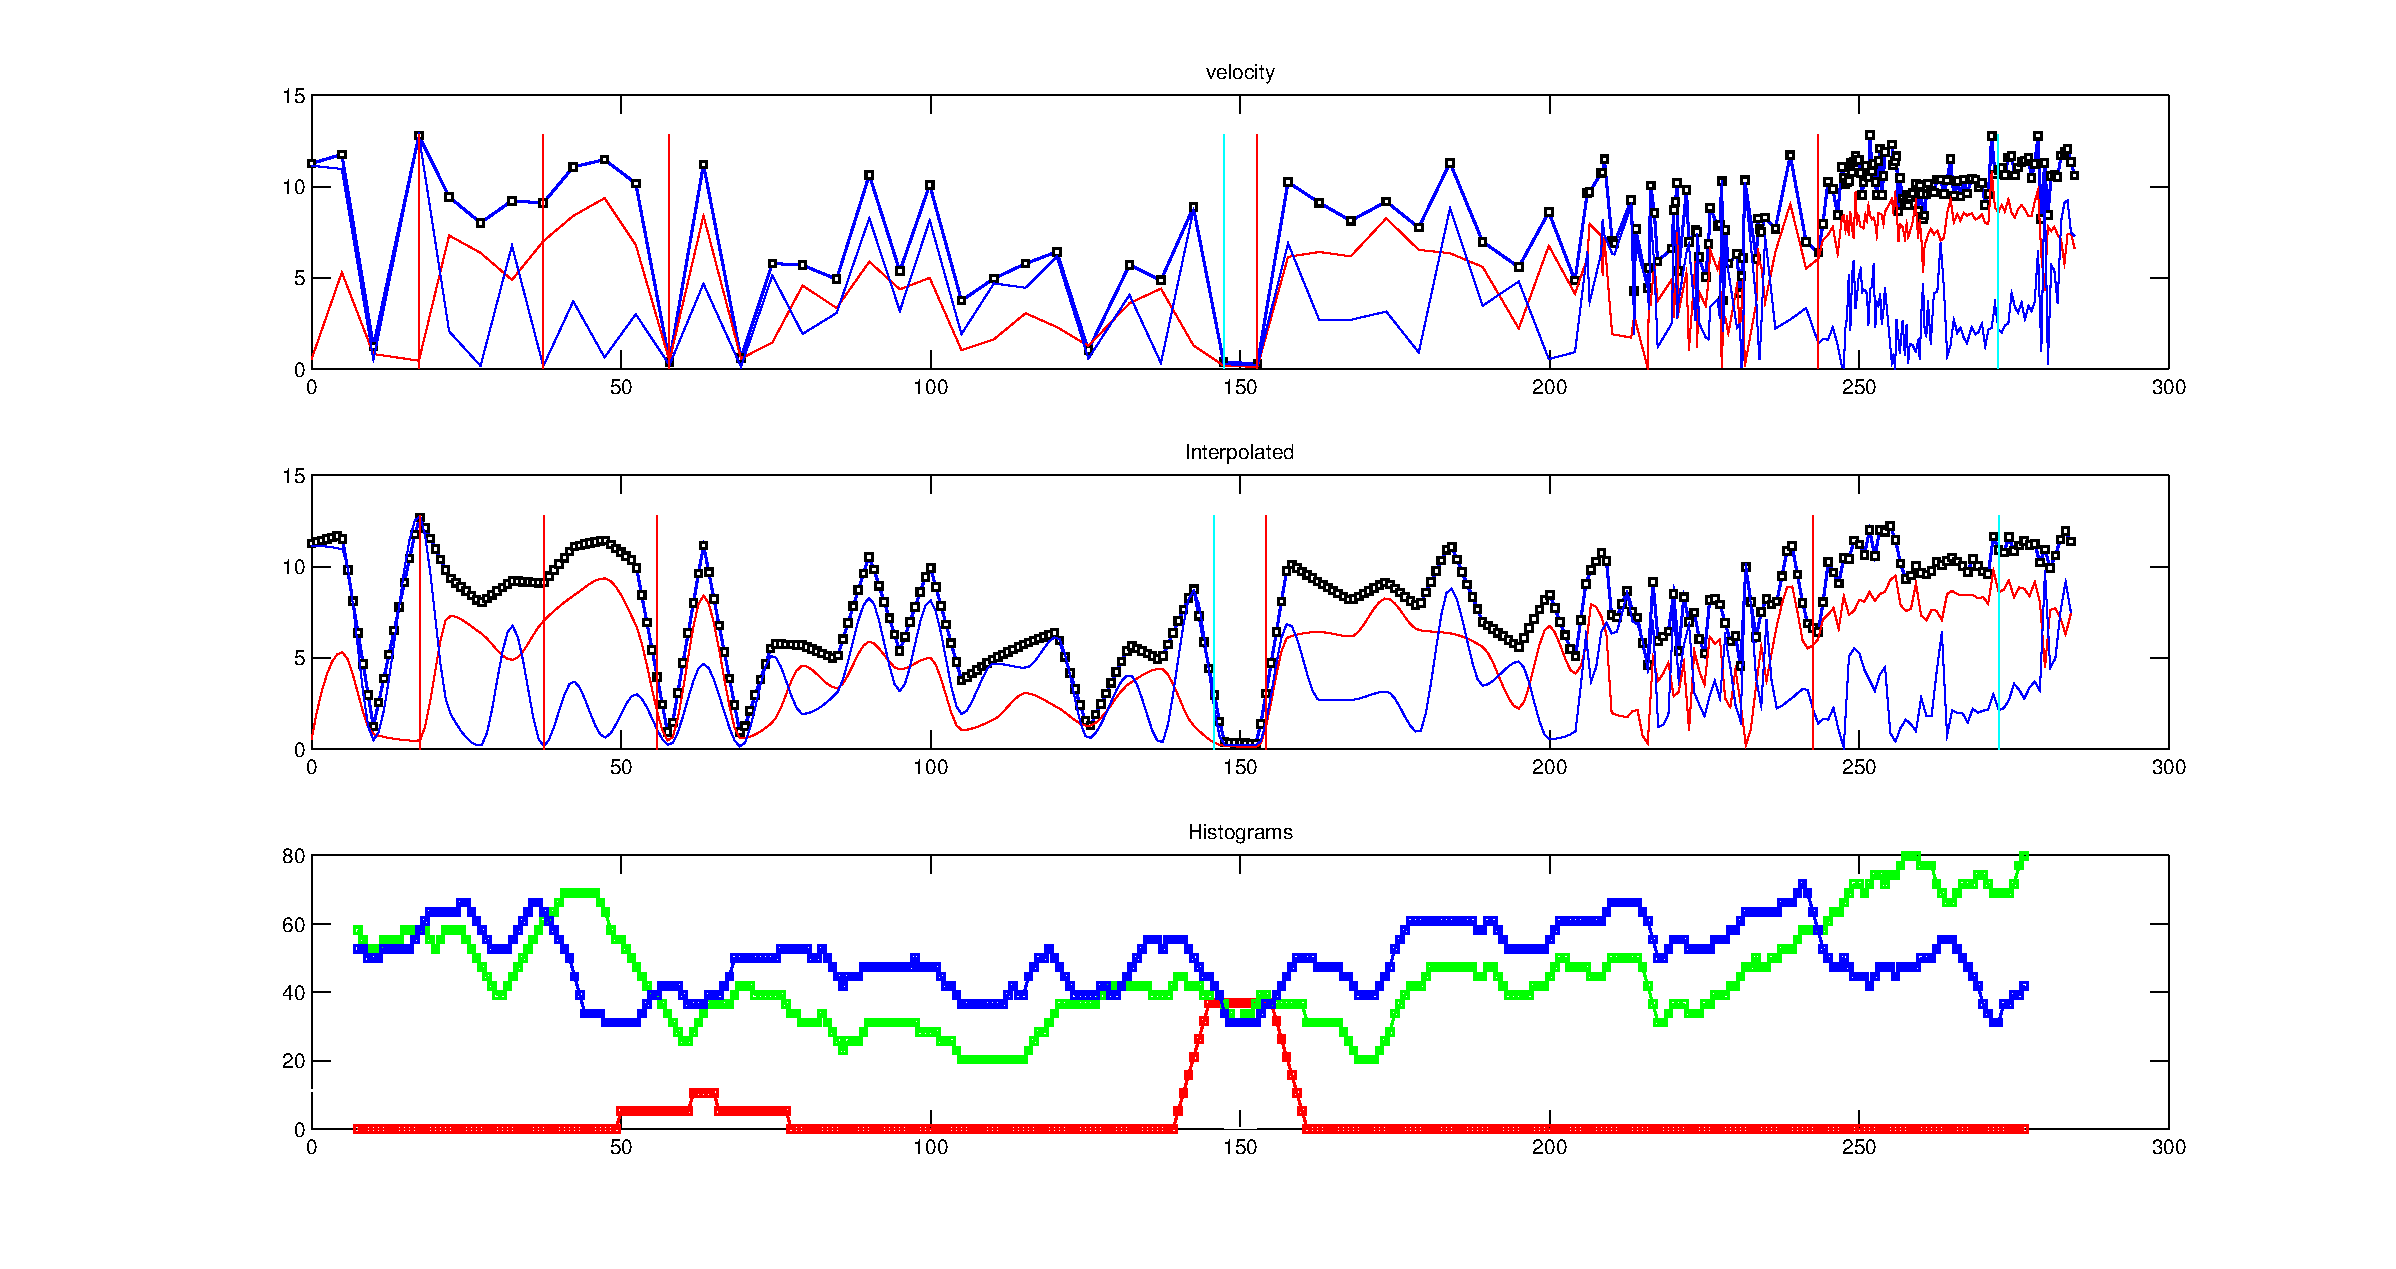
\includegraphics[width=\textwidth]{clustering.pdf}
%\caption{\small How clustering works. Above is the raw data. The marked line is the
%absolute speed of the bird. The red and blue lines under it are the speeds in
%the x and y direction.\\
%The middle image shows the interpolated data.\\
%The bottom image shows how much the point in the middle image resembles a
%certain kind of behavior. Red is floating, green is flying and blue is foraging.}
%\label{fig:clustering}
%\end{figure}

\subsubsection{Smoothing the current data}
After the previous step, the data sometimes has only one or two points above the
others, during a cluster. This could be due to a gps error or a sudden movement
of the bird. We do not want to see this as a new cluster, so the data should be
smoothed.

This is done in a simple and elegant way. A window of (in our case) 7 points is
moved over the data. The mode of these points should be the value of the middle
of the seven. This way, if less than four of the points have another value than
their surroundings, there are too little points to create a new cluster, and the
difference was probably noise. 



 \subsection{Annotating the data}
 % Describes how we annotate (including how the tool works. Maybe an appendix
 % should be added on how the tool should be started and how it should be used.









\section{Learning}



The focus of this report was cluster finding by unsupervised learning, which gave some workable results. The found clusters can be used to identify behaviour using machine learning techniques. We will give an example of how this can be done in a way that is easy to extend. We will use the clusters that we manually labeled and attach a set of features to them (a set of properties that describe it). With the cluster labels and their features we train a learning algorithm and test its accuracy.

 \subsection{Features}
 The features we came up with consist of numeric values and can be derrived from the cluster data. Some are used for manual annotation and some are values that we hope the learning algorithm can use to find hidden relations. Here is a list with their descriptions:

 \begin{description}
  \item[Duration] The duration of the cluster in seconds.
  \item[Average speed] Average speed during the cluster in km/h.
  \item[Height difference] An estimation of the height traveled in meters. The height is very unreliable, even after removing outliers, so we can not just use the sum of the values. Instead we calculate the derivative of the height numerical (the verticale speed) and take the average value. To make this value more intuitive we multiply it by the duration of the cluster, which results in the average vertical distance traveled.
  \item[Ground distance] Distance between cluster begin- and endpoint in km. 
  \item[Total distance] Total distance traveled in km.
  \item[Angle variance] The average change of direction in degrees per minute. On low resolution it can look like the bird is flying in a straight line, while he is really making sharp turns. Figure \ref{fig:anglevar1} shows a bird\footnote{bird 344, session 10} who seems to be flying straight on his trajectory, while his speeds indicate he is not. For this reason we do not use the angle between two data points, but the angle between two \emph{instantaneous speed vectors}. These are 3d vectors indicating the motion of the bird measured on a small time interval.

\begin{figure}[htb!]
\begin{center}
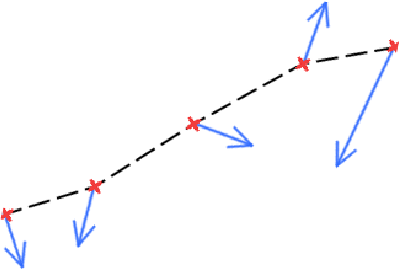
\includegraphics[scale=0.8]{anglevar2.png}
\end{center}
\caption{Trajectory of a bird with his instantaneous speeds} 
\label{fig:anglevar1}
\end{figure}

  There are some problems with this feature, because the instantaneous speed is unreliable. When the resolution is high the time passed between two points is very low, but the angle between them can be a bit jumpy. This results in large changes in angle while the bird is flying straight. We try to limit this error by sampling the data when the resolution is too high (above 1 dat/min is the limit used in our code).
  \item[Distance difference] The difference between \emph{ground distance} and \emph{total distance}. When the bird is hunting he often flies in circles and returns near his startpoint, which is easy to read in this variable (we include this because the learning algorithm can not see spatial information in the trajectory).
  \item[Resolution] The average amount of data points per minute in the clusters data. Not very useful for us but maybe for the learning algorithm.
  \item[Fourier frequencies] Maximum frequency in the fourier transform in the $x$, $y$ and $z$ directions (three features). The fourier transform is an operation that expresses a function of time as a function of frequencies. This is a logical way to express acceleremeter data. For the implementation we used a method called the \emph{Fast Fourier transform}\footnote{TODO Reference to article in repo}. 

  \begin{figure}[htb!]
    \centering
    \subfloat[Accelerometer data, on the x-axis time (ms)]{
      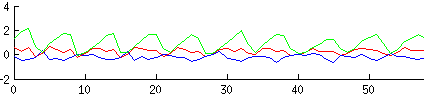
\includegraphics{acc1}
    }\\
    \subfloat[Fourier transform of the above data, on the x-axis frequency (Hz)]{
      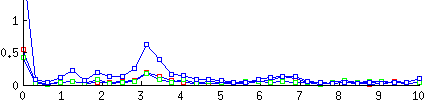
\includegraphics{fourier2}
    }\\
    \caption{The fourier transform on a fragment of accelerometer data}
    \label{fig:fourier}
  \end{figure}

  Figure \ref{fig:fourier} shows an example of a fourier transform on accelerometer data. There is a peak at 3 Hz, which means the accelerometer data has fragments recurring at that frequency. The peak at 0 Hz is an aspect of the Fourier transform and can be ignored. 

  Our fourier transform only returns the maxiumum frequencies of one point of accelerometer data. We currently use the center point for this feature, which is not te best method because that point could contain noise. This could be improved by taking the average of the frequencies of all accelerometer data in the cluster.
  \item[Previous cluster] The id of the previous cluster. This may be needed to recognize some behaviour, like digesting (after hunting).
 \end{description}

 We store the features in a Matlab array and save them to a csv file.

\subsection{Adding Features}
The GPS and accelerometer data can be used to create different features not mentioned above. We did not have the resources to do research in finding the best features, but we wanted to be able to add new ones without re-annotating the data. All features are calculated in \verb|createClusterFeatures.m| and are then saved along with their annotation. When a new feature is thought up it can be appended to the return value of that function. Then \verb|raloadFeatures.m| can be used to recreate the features, transferring all previous annotations. 

 \subsection{Results}
 We then appended all the csv files into a large database of training data. We removed \emph{unknown} and \emph{bad} labeled clusters as they indicate bad clustering or insufficient knowledge of birds. To improve the result we also combined \emph{digesting} and \emph{sleeping} clusters into one class. They can be seperated in future experiments, but with our current features and annotations an algorithm will not find a difference. The training data can then be loaded into a machine learning program. We chose for WEKA\footnote{http://www.cs.waikato.ac.nz/ml/weka/} because it is easy to use and it supports many learning algorithms.

 For the tests we use following dataset:
\begin{itemize}
\item 1637 annotated clusters
\item 12 features
\item 3 classes (Flying, Floating and Diving)
\end{itemize}


WEKA gave the following results, using 10-fold crossvalidation for testing:

\begin{center}
\begin{tabular}{r|c}
	\textnormal{Method} & \textnormal{Precision} \\ \hline 
	Tree J48 & 81\% \\
	Logistic & 82\% \\
  Perceptron & 82\% \\
\end{tabular}
\end{center}


The learning methods yield very similar results. Figure \ref{fig:tree} shows the J48 tree that was generated. 

\begin{figure}
\begin{center}
  \xymatrix{
    && *+<12pt>[F-:<12pt>]{\txt{avgSpeed}}\ar[dl]|{<=12.315}\ar[dr]|{>12.315}  & & & &\\
    &*+<12pt>[F=:<12pt>]\txt{floating} & & *+<12pt>[F-:<12pt>]\txt{grndDist}\ar[dl]|{<=2.6718}\ar[dr]|{>2.6718} & &\\
    && *+<12pt>[F-:<12pt>]\txt{distDiff}\ar[dl]|{<=0.10189}\ar[dr]|{>0.10189} & & *+<12pt>[F=:<12pt>]\txt{flying} &\\
    &*+<12pt>[F=:<12pt>]\txt{flying} & & *+<12pt>[F-:<12pt>]\txt{grndDist}\ar[dl]|{<=1.1718}\ar[dr]|{>1.1718} & &\\
    && *+<12pt>[F=:<12pt>]\txt{diving} & & *+<12pt>[F-:<12pt>]\txt{angleVar}\ar[dl]|{<=0.1878}\ar[dr]|{>0.1878}\\
    && & *+<12pt>[F=:<12pt>]\txt{flying}& & *+<12pt>[F-:<12pt>]\txt{distDiff}\ar[dl]|{<=0.6530}\ar[dr]|{>0.6530} & \\
    && & & *+<12pt>[F=:<12pt>]\txt{flying}& & *+<12pt>[F=:<12pt>]\txt{diving}
  }
  \caption{Visualisation of the decision tree generated by WEKA}
  \label{fig:tree}
\end{center}
\end{figure}

Most of the errors were made in classifying \emph{diving}, the cunfusion matrix shows this:
\begin{verbatim}
=== Confusion Matrix ===

   a   b   c   <-- classified as
 519  26  22 |   a = floating
  35 632  77 |   b = flying
  64  99 163 |   c = diving
\end{verbatim}
The following table shows the prediction accuracy for each class:
\begin{center}
\begin{tabular}{l|l}
	\textnormal{Class} & \textnormal{Correctly classified} \\ \hline 
	Floating & 91.5\% \\
	Flying &  85.1\% \\
	Diving & 50.0\% \\
\end{tabular}
\end{center}

When annotating by hand it was also difficult to distinguish diving, escpecially on low resolution. The data used was annotated by 4 different people with little knowledge of birds, we suspect this is the bottleneck for the accuracy. 

\section{Conclusions and results}

\section{Improvements and future work}
test


\end{document}
